% !TeX spellcheck = en_US
% !TeX encoding = UTF-8
\chapter{Conclusion}
\section{Discussion}

Discussion of the results compared to the objective--- Limitation(sujective ground thruth)---- Future work(improvement in detection model, real time system schematic and breif, parameter tuning of the controller etc etc)
and then conclusion


\section{Analysis of ground truth}

\begin{figure}[!htbp]
	\centering
	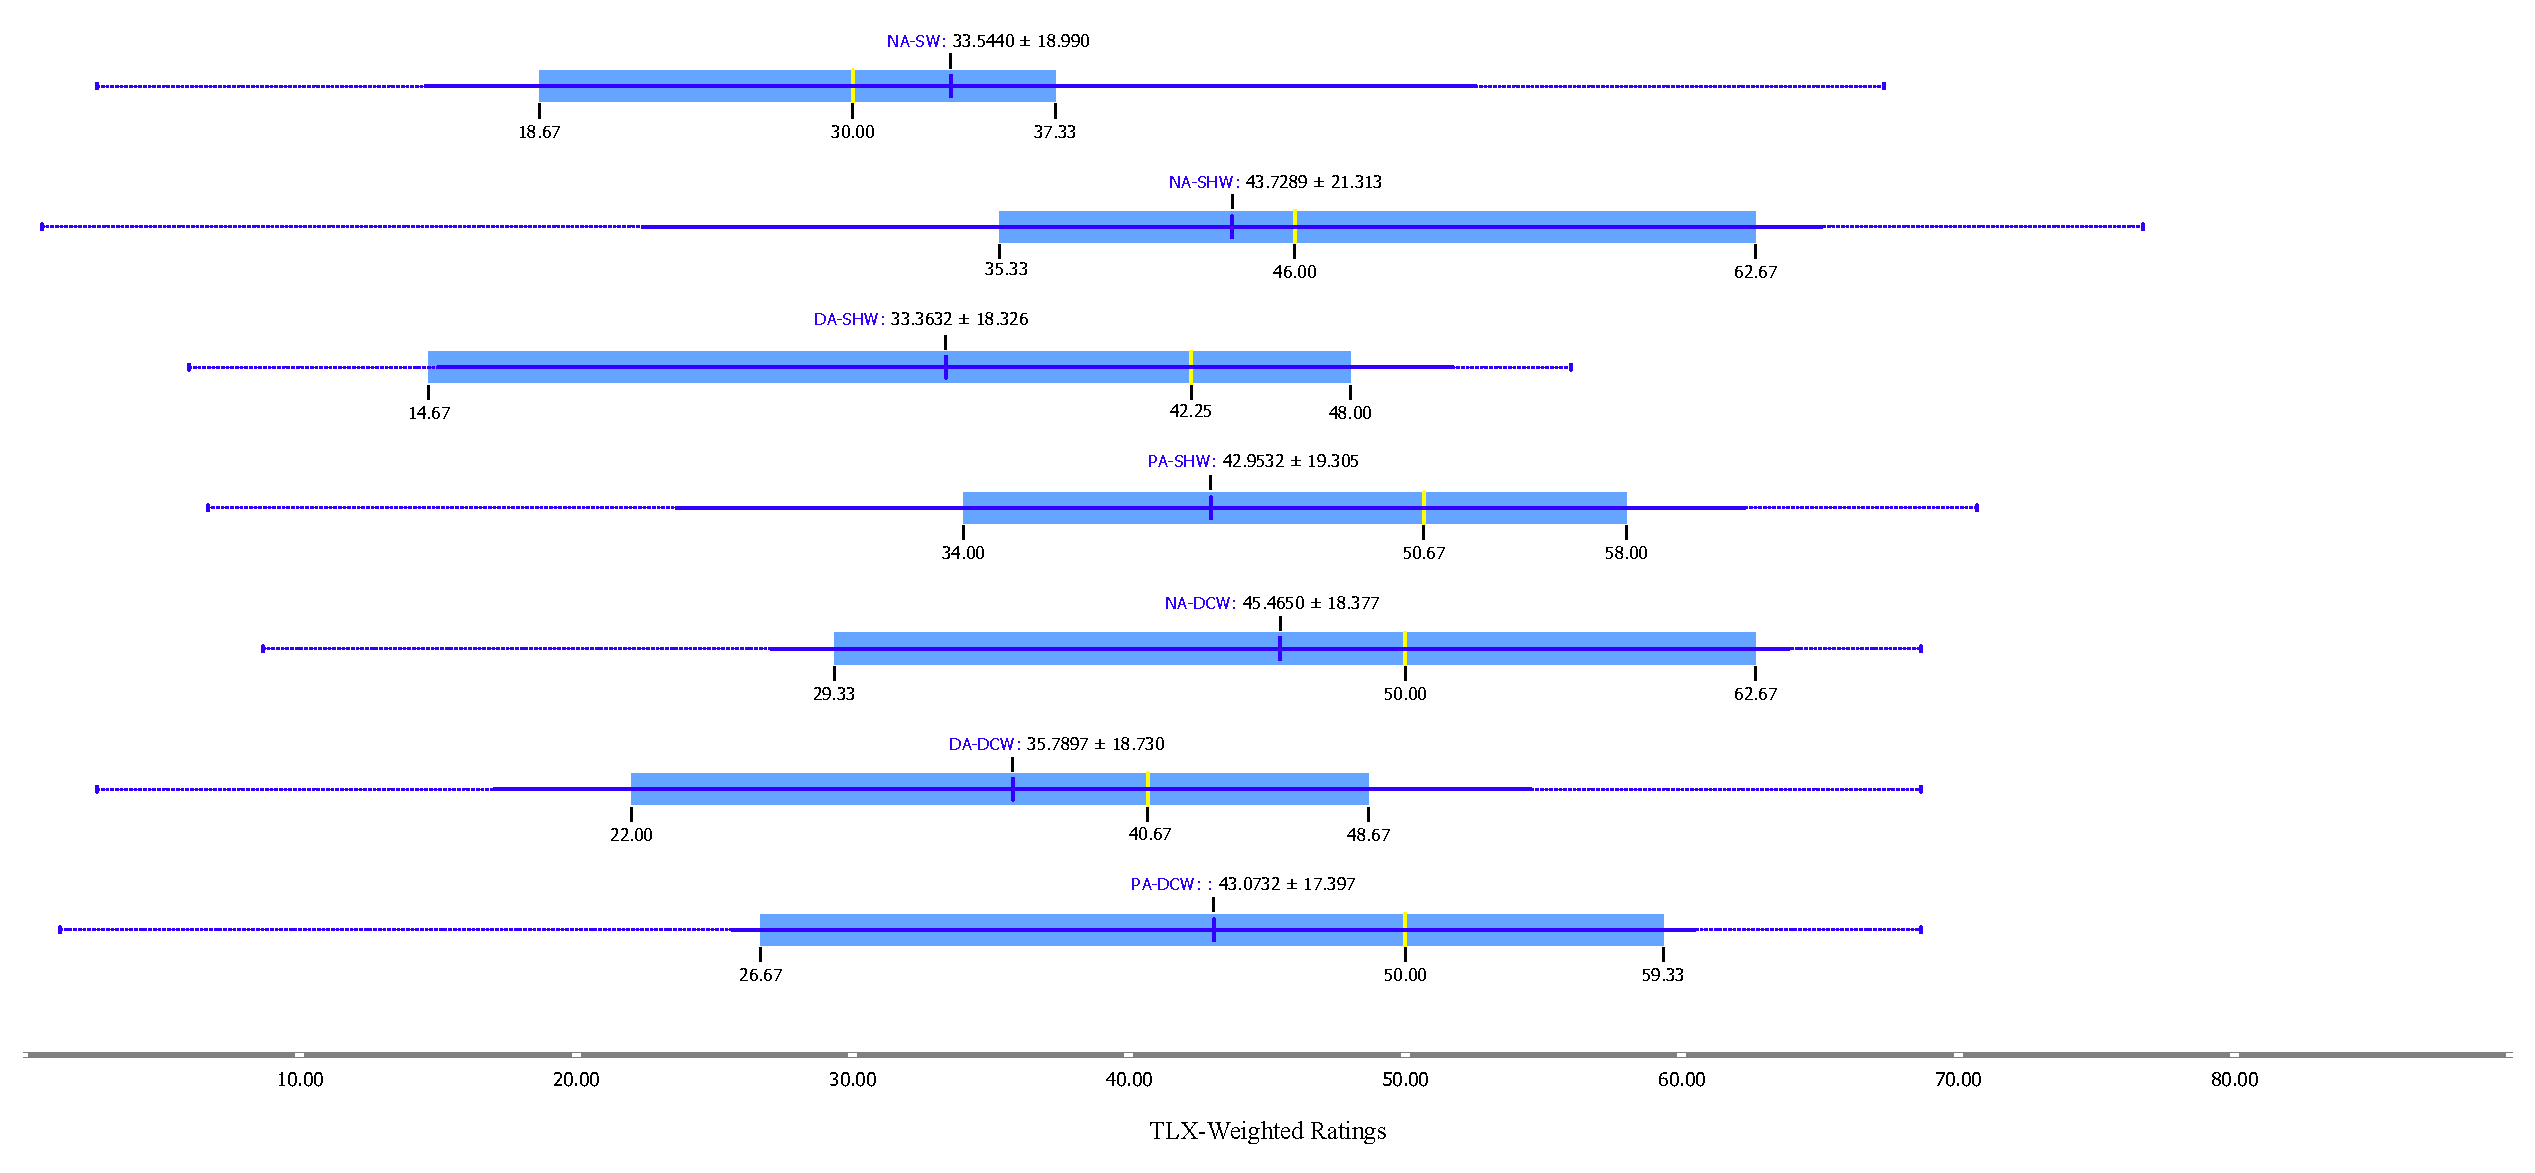
\includegraphics[width=\columnwidth]{images/tlx.pdf}
	\caption{}
	\label{fig:netwrok}
\end{figure}

In our research on stress analysis, we primarily relied on subjective measures for labeling and establishing ground truth. While many previous studies have successfully employed this approach, it is important to acknowledge that subjective ratings can be influenced by a variety of factors. These influences could range from individual perception differences to contextual and environmental factors impacting a participant's response. Consequently, reducing the complex and multifaceted nature of stress into a three-class system based on subjective assessments might lead to oversimplifications of the nuanced nature of stress.


To bolster the reliability of our labeling process, we undertook an initiative to crossvalidate our labels with other physiological or behavioral stress indicators. This crossvalidation aimed to correlate our subjective stress labels with objective measures, such as mean skin conductance response meanscr and heart rate meanhr. It is crucial to note that this assumption that meanscr and meanhr directly indicate stress was specifically for the purpose of this crossvalidation exercise and not a general assumption throughout our project.


Given that physiological features like meanscr and meanhr are integral inputs of our stress detection model, they could not be directly used for labeling the stress categories. This constraint necessitated our reliance on subjective measures for labeling. However, by attempting to correlate these objective physiological indicators with our subjective labels, we sought to add a layer of validation to our approach.


Before delving into our results, it is imperative to discuss some critical caveats about our methodology. Our reliance on subjective ratings, though methodologically sound in many aspects, does not entirely capture the reliable ground truth of stress. The subjective nature of these ratings means they are susceptible to various influencing factors, which might not always align perfectly with physiological manifestations of stress. This acknowledgment is crucial for a comprehensive understanding of our findings and their interpretation.


Our approach, while aligned with standard practices in stress research, does acknowledge the limitations inherent in using subjective measures for stress categorization. By attempting cross-validation with physiological data, we endeavored to enhance the robustness of our methodology. Nevertheless, the complexities and intricacies of stress as a psychological and physiological phenomenon demand careful consideration and interpretation of our results.


\section{Future work}

%\section{Latex distributions and editors}